\chapter{Modelo alternativo}

\label{ch:modelo_alternativo}

\section{Introducción}

Como adelantábamos en la sección 1.3 si nos centramos en el modelado BEWARE de la transcripción génica esencialmente tenemos dos enfoques: modelar la expresión génica como una cantidad proporcional a la suma ponderada de los factores de transcripción o hacerlo proporcional a la probabilidad de unión del ARN polimerasa, que va modificada por los factores de transcripción.

Tras extenso estudio que se ha hecho del modelo \cite{schaffer}, la multiestabilidad está más que demostrada para conjuntos de valores de parámetros esperables, así como para un conjunto de condiciones iniciales que tambien podrían esperarse en situaciones biologicas. 

Sin embargo, debido a esto (la multiestabilidad que se pone de manifiesto en el estudio del modelo) sabemos que este modelo debe ser modificado, puesto no tiene un soporte experimental biológico contrastado.

Es decir, en experimentos biológicos no observamos este tipo de multiestabilidad. Por tanto si queremos que nuestro modelo de transcripción represente fielmente el comportamiento de la transcripción genetica debemos modificarlo o cambiarlo.

Así, antes de cambiar grandes características de nuestro modelo, nace la idea de modificar nuestra forma de crear el operador BEWARE usando el segundo enfoque que tiene en cuenta el ARN polimerasa. 

Tras el esquema de modelado, vamos a presentar los experimentos numéricos que nos llevan a pensar que podemos estar ante un comportamiento más fiel a lo observado en biología con sólo un estado estable. 

\section{Modelado BEWARE}
Comenzamos aplicando las ideas del método termodinámico a nuestros dos genes, gli y ptc, los cuales suponemos controlados por tres factores de transcripción $\{Gli, Gli_3, Gli3R\} $ que son activador, activador y represor, respectivamente.

\subsubsection{Consideraciones inciales}
\begin{itemize}

\item Destacamos de nuevo, antes de comenzar el resto del calculo del operador, que la expresión de la evolución de la cantidad de las proteínas generadas por gli y ptc, Gli y Ptc, vendrá disminuida por la degradación natural de estas moléculas con dos constantes de degradación. Esto implica que nuestro resutlado final será un modelo de la forma:
\begin{equation}
\frac{dGli}{dt}=BEWARE([Gli],[Gli_3],[Gli3R])-k_{deg}Gli
\label{expr}
\end{equation}
e igual con el Ptc.

\item En el modelo, además, las reacciones de unión de los factores de transcripccón y del ARN polimerasa son mucho más rápidos que la síntesis de la proteína Gli o Ptc, por lo tanto, consideramos en equilibrio termodinámico dado por la Ley de Acción de Masas.

\item Por otra parte en este trabajo se considera una versión del operador con cooperatividad total/ausencia de cooperatividad entre factores de transcripción. Podríamos estudiar cómo afecta la hipótesis de tener una cooperatividad parcial en futuros desarrollos del mismo, siguiendo las indicaciones de \cite{cambon1}.
	 
\end{itemize}
Todos los pasos siguen el esquema general presentado en \cite{cambon1}:
\subsection{Calculo del operador}
Nuestro objetivo es averiguar la expresión del operador BEWARE en \ref{expr}.
Partiendo de la segunda consideración inicial, calculamos la expresion de los primeros complejos que se formarían al unir a una region de regulación vacía ([B] de ahora en adelante) con alguno de los promotores ($Gli$ y $Gli_3$), represores (Gli3R) o ARN polimerasa. En ese caso, tienen una concentración en el equilibrio termodinámico expresada como:

\begin{equation}
[BW]=\frac{K^{(1)}_{+W}}{K^{(1)}_{-W}}[W][B]:=\frac{[W]}{K^{(1)}_W}[B]
\end{equation}

donde W representa cualquier activador, represor o ARN polimerasa y $K^{(1)}_W$ es la constante de disociación. Además, siguiendo la notacion de \cite{cambon1}, el superindice (1) representa que no hay otro factor de transcripcion en el momento de la union en el complejo. 

Nuestro enfoque principal ocurre en una situación de cooperatividad\footnote{Si se produce la cooperación, sería necesario saber qué factores de transcripcion se ven afectados por otros puesto que el  la concentración del equilibrio dependerá de estas relaciones. En nuestro caso particular, sí podemos usar este enfoque.}. Por tanto, cuando nuevos factores se unan al complejo su constante de disociación vendrán modificada por los anteriores. Esto es, sea la reaccion
\begin{equation}
\ce{[W] + [BW] <->[k^{(2)}_{+W}] [BWW] }
\label{s:125}
\end{equation}
las concentraciones de equlibrio cendrían dadas siguiendo el equilibrio termodinamico:

\begin{equation}
[BWW]=\frac{[W][W]}{K_{W}^{(2)}K_{W}^{(1)}}[B]
\end{equation}


sin embargo, la cooperatividad se refleja si imponemos que, para $i,k= Gli,Gli3,Gli3R,ARNP$ :
$$K_i^{(2)}=K_k^{(1)}/c
$$
donde c es una constante positiva mayor que 1. En particular, nuestro modelado está enmarcado en la situacion de cooperatividad total, esto implica que cuando se une un factor de transcripcion a nuestro complejo este modifica las afinidades de todos los siguientes de la misma manera.


Notemos n el número de posiciones de union ( en nuestro caso n=3) de namera que $j_A$ sea el numero de activadores unidos ($j_{gGi}+j_{Gli_3}$), $j_r=j_{GliR3}$ el numero de represores y $j_0=n-j_A-j_R$ como el numero de espacios libres.  

Con ello, para calcular el estado de equilibrio de cualquier disposicion, tenemos:
\begin{equation}
[BGli^{j_{Gli}}Gli_3^{j_{Gli_3}}Gli3R^{j_{Gli3R}}]=[B]c^{(j_A+j_R-1)_+}\left(\frac{[Gli]}{K_{Gli}}\right)^{j_{gli}}
\left(\frac{[Gli_3]}{K_{Gli_3}}\right)^{j_{gli_3}}
\left(\frac{[Gli3R]}{K_{Gli3R}}\right)^{j_{gli3R}}
\label{eqa}
\end{equation}
Donde + denota la funcion parte positiva, puesto que la cooperatividad no tiene lugar si no hay 2 o mas factores de transcripcion cooperativos en la configuracion.

Con respecto al proceso de unión de ARN polimerasa, los factores de transcripcion trabajan juntos tratando de activar o reprimir el proceso de union por un mecanismo conocido como reclutamiento. 

Por lo tanto, consideramos que los activadores interactúan con RNAP con
una interacción 'adhesiva' que da lugar a una modificación de la afinidad de la unión de la ARN polimerasa: $K_{RP} / a^{j_A}$ donde $a$ es una constante de cooperatividad mayor que 1.
 
Por el contrario, el efecto de los represores se modela en términos de una interacción "repulsiva" que modifica el afinidad de unión  $K_{RP} / r^{j_R}$ con un factor anti-cooperatividad r menor que 1.

\subsubsection{Espacio de todas las configuraciones}
Para avanzar en la obtención del operador BEWARE siguiendo el esquema, comenzamos calculando el espacio de todas las posibles configuraciones.
Sea un complejo compuesto por $j_{Gli}, j_{Gli_3}, j_{Gli3R}, j_0, j_P$ activadores, represores, espacios vacíos y ARN polimerasa. En particular $j_p$ puede ser 0 o 1 según encontremos o no ARNp en el compuesto.

Supongamos que no hay ningun ARN polimerasa en nuestro complejo (esto es, $j_p=0$). En ese caso el estado de equilibrio vendría dado por la expresión:
\begin{equation}
\textit{C}(C)[B]
\left(\frac{[Gli]}{K_{Gli}}\right)^{j_{gli}}
\left(\frac{[Gli_3]}{K_{Gli_3}}\right)^{j_{gli_3}}
\left(\frac{[Gli3R]}{K_{Gli3R}}\right)^{j_{gli3R}}
\end{equation}
donde $\textit{C}(C)$ hace referencia a $c^{(j_A+j_R-1)_+}$. Además, como hemos dicho, nuestro modelo no tiene en cuenta la disposición espacial, con lo que este estado puede venir dado por todas las combinaciones espaciales del numero de activadores, represores y espacios vacíos que nos indica $j_{Gli}, j_{Gli_3}, j_{Gli3R}, j_0$. Por tanto, multiplicamos este estado por todas la combinaciones que pueden darle lugar a él. Esta cantidad viene dada por simple combinatoria: $$\frac{3!}{j_{Gli}! j_{Gli_3}! j_{Gli3R}! j_0!}$$.

Tenemos por tanto, la expresión de todas las configuraciones de equilibrio sin el papel del ARNp:
\begin{equation}
\begin{split}
&Z^{(3)}(j_{Gli}, j_{Gli_3}, j_{Gli3R},j_P=0;C)=\\&=\textit{C}(C)\frac{3!}{j_{Gli}! j_{Gli_3}! j_{Gli3R}!j_0!}[B]\frac{[RNAP]}{K_{RP}}
\left(\frac{[Gli]}{K_{Gli}}\right)^{j_{gli}}
\left(\frac{[Gli_3]}{K_{Gli_3}}\right)^{j_{gli_3}}
\left(\frac{[Gli3R]}{K_{Gli3R}}\right)^{j_{gli3R}}
\end{split}
\end{equation}

 Supongamos ahora que el ARN está en nuestro complejo (esto es, $j_p=1$).
 De nuevo vamos a tener unos espacios ocupados y otros vacíos, dados por: $j_{Gli}, j_{Gli_3}, j_{Gli3R}, j_0$.
 
Todas las formas posibles configuracione para obtener una concentración de equilibrio con $j_{Gli}, j_{Gli_3}, j_{Gli3R},j_P$ activadores, represores de nuevo se obtienen con la misma expresion. 
Sin embargo, ahora tenemos en cuenta el valor que aporta el ARNp. Siguiendo lo expuesto en los preliminares, la existencia de activadores y represores, modifica la afinidad de union del ARN. Tenemos por tanto que el factor del ARNp dentro de nuestro complejo, en ausencia de factores viene expresado como: 
\begin{equation}
[B.ARNp]=\frac{[ARNp]}{K_{RP}}[B]
\end{equation}
 En caso de que existan factores de transcripcion tenemos que modificar la afinidad según comentabamos:
 \begin{equation}
 \frac{K_{RP}}{a_{Gli}^{j_{Gli}}a_{Gli3}^{j_{Gli3}}r_{Gli3R}^{j_{Gli3R}}}
 \end{equation}
  Donde $a_{Gli}a_{Gli3}r_{Gli3R}$ son las constante de cooperatividad y anticooperatividad asociadas a los factores de transcripción (y aparecen en la expresión modificadas según el numero de cada una, lo cual viene indicado en el exponente)
  
  Tenemos pues la expresión para describir el estado:
\begin{equation}
\textit{C}(C)\frac{3!}{j_{Gli}! j_{Gli_3}! j_{Gli3R}!j_0!}[B]\frac{[RNAP]a_{Gli}^{j_{Gli}}a_{Gli3}^{j_{Gli3}}r_{Gli3R}^{j_{Gli3R}}}{K_{RP}}
\left(\frac{[Gli]}{K_{Gli}}\right)^{j_{gli}}
\left(\frac{[Gli_3]}{K_{Gli_3}}\right)^{j_{gli_3}}
\left(\frac{[Gli3R]}{K_{Gli3R}}\right)^{j_{gli3R}}
\end{equation}

 Agrupando por exponentes, podemos obtener la expresión final:
\begin{equation}
\begin{split}
&Z^{(3)}(j_{Gli}, j_{Gli_3}, j_{Gli3R},j_P=1;C)=\\&=\textit{C}(C)\frac{3!}{j_{Gli}! j_{Gli_3}! j_{Gli3R}!j_0!}[B]\frac{[RNAP]}{K_{RP}}
\left(\frac{a_{gli}[Gli]}{K_{Gli}}\right)^{j_{gli}}
\left(\frac{a_{gli_3}[Gli_3]}{K_{Gli_3}}\right)^{j_{gli_3}}
\left(\frac{r_{gli3R}[Gli3R]}{K_{Gli3R}}\right)^{j_{gli3R}}
\end{split}
\end{equation}

Esto nos permite describir todo el espacio muestral, es decir, el espacio de todas las posibles configuraciones, atendiendo al numero de factores de transcripción y a la existencia o no de ARN polimerasa:
\begin{equation}
\Omega=\{(j_{Gli}, j_{Gli_3}, j_{Gli3R},j_P);j_{Gli}, j_{Gli_3}, j_{Gli3R}\geq0;j_{Gli}+ j_{Gli_3}+ j_{Gli3R}\leq 3,j_p=0,1\}
\end{equation}


\subsubsection{Definicion de la probabilidad de cada configuración}

Una vez que hemos descrito todas las configuraciones posibles en términos de las concentraciones de activador Gli y Gli3, del represor Gli3R y ARN polimerasa, obtenemos fácilmente la probabilidad de encontrar el promotor en una configuración particular de $j_P$ ARN polimerasa y de factores de transcripcion $j_{Gli}, j_{Gli_3}, j_{Gli3R}$ relacionados por una cooperatividad $c$.

\begin{equation}
P^{(3)}(j_{Gli}, j_{Gli_3}, j_{Gli3R},j_P;C)=\frac{Z^{(3)}(j_{Gli}, j_{Gli_3}, j_{Gli3R},j_P;C)}{\sum_{\{j'_{Gli}, j'_{Gli_3}, j'_{Gli3R},j'_P\}\in\Omega}Z^{(3)}(j'_{Gli}, j'_{Gli_3}, j'_{Gli3R},j'_P;C)}
\label{probabilidad}
\end{equation}
 con $(j_{Gli}, j_{Gli_3}, j_{Gli3R},j_P)\in\Omega$
 
\subsubsection{Resultado final del operador BEWARE}
\begin{equation}
\begin{split}
&BEWARE([Gli][Gli_3][Gli3R][ARNP];C)=\\&=C_B\sum_{j_{Gli}, j_{Gli_3}, j_{Gli3R}\geq0}^{j_{Gli}+ j_{Gli_3}+ j_{Gli3R}\leq n}P^{(n)}(j_{Gli}, j_{Gli_3}, j_{Gli3R},j_P=1;C)
\end{split}
\end{equation}
Al dividir el denominador en dos sumas, segun la ARN polimerasa este ligada o no a la configuración, esta expresión puede reescribirse en términos de la función del factor de regulación, $F_{reg}$:
\begin{equation}
BEWARE(Gli, Gli_3, Gli3R)=\frac{c_{b}}{1 + \frac{k_{RNAP}}{F_{reg}(Gli, Gli_3, Gli3R) RNAP}},
\end{equation}

Realizando los calculos indicados en \cite{cambon1}, vía el paquete \cite{sympy}, este factor de regulación se puede reducir para facilitar el
comprensión del proceso general. Se obtiene así, la expresion:
\begin{equation}
F_{reg}([Gli][Gli_3][Gli3R];C)=\frac{S^{(3)}(a_{Gli}[Gli]K_{Gli}^{-1},a_{Gli_3}[Gli_3]K_{Gli_3}^{-1},r_{Gli3R}[Gli3R]K_{Gli3R}^{-1};C)}{S^{(3)}([Gli]K_{Gli}^{-1},[Gli_3]K_{Gli_3}^{-1},[Gli3R]K_{Gli3R}^{-1};C)}
\end{equation}

donde $S^{(3)}(x,y,z;C)$ viene dads por la cooperatividad total que hemos asumido:
\begin{equation}
S^{(3)}(x,y,z;C)=1 + \frac{1}{c} \left(1+cx+cy+cz\right)^{3} - \frac{1}{c}
\end{equation}

Concluimos así el calculo del modelado del operador BEWARE con un enfoque estimulated. Con este operador y las ecuaciones definidas en el capítulo 1 podemos disponer ya de nuestro modelo completo.

\section{Sistema final}

La mayoría de cuentas del apartado se han generado con la ayuda de \cite{sympy}.

\begin{equation}
\frac{dGli}{dt} = BEWARE(Gli, Gli_3, Gli3R)-k_{deg}Gli,
\label{equ:12}
\end{equation}

\begin{equation}
\frac{dGli_3}{dt} = \frac{r_{g3b}}{Ptc}-Gli_3\left(k_{deg}+\frac{k_{g3rc}}{K_{g3rc}+Signal}\right),
\label{eq:22}
\end{equation}

\begin{equation}
\frac{dGli3R}{dt}= Gli_3\left(\frac{k_{g3rc}}{K_{g3rc}+Signal}\right)-k_{deg}Gli3R,
\label{eq:32}
\end{equation}

\begin{equation}
\frac{dPtc}{dt} = BEWARE(Gli, Gli_3, Gli3R)-k_{degp}Ptc.
\label{eq:42}
\end{equation}


Donde tenemos, por definición:
 \begin{equation}
Signal=\frac{\frac{Shh}{k_{shh}} + 1}{\frac{Shh}{k_{shh}} + 1 + \frac{Ptc}{k_{ptc}}},
\label{signal} \end{equation}

y,


\begin{equation}
BEWARE(Gli, Gli_3, Gli3R)=\frac{c_{b}}{1 + \frac{k_{RNAP}}{F_{reg}(Gli, Gli_3, Gli3R) RNAP}},
\end{equation}

donde solo nos queda describir $F_{reg}$. En el caso de de gradientes opuestos y no/total cooperatividad de los factores de transcripción nos queda:

\begin{equation}
F_{reg}=\frac{1 + \frac{1}{c} \left(\frac{Gli a_{Gli}}{k_{Gli}} c + \frac{Gli_{3} a_{Gli3}}{k_{Gli3R}} c + \frac{Gli3R c}{k_{Gli3R}} r_{Gli3R} + 1\right)^{3} - \frac{1}{c}}{1 + \frac{1}{c} \left(\frac{Gli c}{k_{Gli}} + \frac{Gli_{3} c}{k_{Gli3R}} + \frac{Gli3R c}{k_{Gli3R}} + 1\right)^{3} - \frac{1}{c}}
\end{equation}






Podemos desarrollar las funciones en cada uno de los términos, quedándonos las siguientes expresiones:
\begin{equation}
\frac{dGli}{dt}=- Gli k_{deg} + \frac{c_{b}}{1 + \frac{k_{RNAP} \left(1 + \frac{1}{c} \left(\frac{Gli c}{k_{Gli}} + \frac{Gli_{3} c}{k_{Gli3R}} + \frac{Gli3R c}{k_{Gli3R}} + 1\right)^{3} - \frac{1}{c}\right)}{RNAP \left(1 + \frac{1}{c} \left(\frac{Gli a_{Gli}}{k_{Gli}} c + \frac{Gli_{3} a_{Gli3}}{k_{Gli3R}} c + \frac{Gli3R c}{k_{Gli3R}} r_{Gli3R} + 1\right)^{3} - \frac{1}{c}\right)}}.
\end{equation}


\begin{equation}
\frac{dGli_3}{dt}=- Gli_{3} \left(k_{deg} + \frac{k_{g3rc}}{K_{g3rc} + \frac{\frac{Shh}{k_{shh}} + 1}{\frac{Shh}{k_{shh}} + 1 + \frac{ptc}{k_{ptc}}}}\right) + \frac{r_{g3b}}{ptc}.
\end{equation}

\begin{equation}
\frac{dGli3R}{dt}=Gli_{3} \left(- Gli3R k_{deg} + \frac{k_{g3rc}}{K_{g3rc} + \frac{\frac{Shh}{k_{shh}} + 1}{\frac{Shh}{k_{shh}} + 1 + \frac{ptc}{k_{ptc}}}}\right).
\end{equation}

\begin{equation}
\frac{dPtc}{dt}=\frac{c_{b}}{1 + \frac{k_{RNAP} \left(1 + \frac{1}{c} \left(\frac{Gli c}{k_{Gli}} + \frac{Gli_{3} c}{k_{Gli3R}} + \frac{Gli3R c}{k_{Gli3R}} + 1\right)^{3} - \frac{1}{c}\right)}{RNAP \left(1 + \frac{1}{c} \left(\frac{Gli a_{Gli}}{k_{Gli}} c + \frac{Gli_{3} a_{Gli3}}{k_{Gli3R}} c + \frac{Gli3R c}{k_{Gli3R}} r_{Gli3R} + 1\right)^{3} - \frac{1}{c}\right)}} - k_{deg p} Ptc.
\end{equation}




\section{Estados estacionarios}\label{apartado3.4}
Siguiendo con el estudio estandar que se lleva a cabo en los modelos matemáticos procedemos con un estudio sobre los estados estacionarios que podemos encontrar en nuestro modelo. En primer lugar procedemos afrontando el problema desde una perspectiva analítica. 

Sean las ecuaciones \ref{equ:12}\ref{eq:22}\ref{eq:32}\ref{eq:42}, si suponemos que éstas se encuentran en un estado estacionario entonces sus cantidades son constantes. Esto implica que su derivada temporal es igual a cero.

Dado que las ecuaciones continen términos complejos, nos interesamos por agruparlas, de manera que los cálculos no sean más sencillo en un primer intento de extraer información:

Por un lado de \ref{equ:12} y \ref{eq:42}:

$$\begin{cases} 0 = BEWARE-k_{deg}Gli, \\0= c_bBEWARE-k_{degp}Ptc. \end{cases}$$
Teniendo en cuenta:

$$
r_{bas,G}=\frac{v_{max,G}}{100},r_{bas,P}=\frac{v_{max,P}}{100}
$$

Si igualamos ambas ecuaciones nos queda:
\begin{equation*}
k_{deg}Gli=BEWARE=\frac{k_{degp}}{c_b}Ptc \implies \frac{k_{deg}}{c_bk_{degp}}Gli=Ptc
\end{equation*}

En particular si llamamos $k_{cc}=\frac{k_{deg}}{c_bk_{degp}}$:
\begin{equation}
k_{cc}Gli=Ptc
\label{gli-ptc2}
\end{equation}


Por otra parte, de \ref{eq:22} y \ref{eq:32}:



$$\begin{cases} 0 = \frac{r_{g3b}}{Gli}-Gli_3\left(k_{deg}+\frac{k_{g3rc}}{K_{g3rc}+Signal}\right), \\0=Gli_3\left(\frac{k_{g3rc}}{K_{g3rc}+Signal}\right)-k_{deg}Gli3R. \end{cases}$$

Sumando, obtenemos:

\begin{equation}
\begin{split}
0=\frac{r_{g3b}}{Gli}-Gli_3k_{deg}-k_{deg}Gli3R & \implies \frac{r_{g3b}}{Gli}=Gli_3k_{deg}+k_{deg}Gli3R\implies
\\
& \implies \frac{r_{g3b}}{Gli_3k_{deg}+k_{deg}Gli3R}=Gli
\end{split}
\label{gli3gli2}
\end{equation}

Con estas cuentas, podemos obtener, en primer lugar, una función de $Signal$\ref{signal} modificada gracias a \ref{gli-ptc2}, la llamaremos $Signal_{modificada}$:
\begin{equation}
Signal_{modificada}=\frac{\frac{Shh}{k_{shh}} + 1}{\frac{Shh}{k_{shh}} + 1 + \frac{k_{cc}}{k_{ptc}Gli}}.
\end{equation}

Ahora, sustituimos los valores que tenemos de manera que podamos expresar todas las concentraciones en función de Gli. 

Nuestro obejtivo es intentar hallar los estados estacionarios mediante los puntos fijos entre dos expresiones de Gli. Con ello, usando \ref{gli3gli2} nos quedaría:

\begin{equation}
\frac{r_{g3b}}{Gli}=Gli_3k_{deg}+k_{deg}Gli3R
\implies Gli_3=\frac{r_{g3b}(K_{g3rc}+Signal_{modificada})}{k_{deg}(K_{g3rc}+Signal_{modificada})Gli}
\label{equgli32}
\end{equation}
Y de nuevo, por  \ref{gli3gli2}:

\begin{equation}
Gli3R=\frac{r_{g3b}}{k_{deg}Gli}-Gli_3
\label{equgli3r2}
\end{equation}

Debido a la capacidad de expresar Gli3R y $Gli_3$ con respecto a Gli, podemos obtener la variación de Promoter y Basal directamente con Gli, substituyendo en ellos el valor de Gli3R y $Gli_3$
Con ello, finalmente obtenemos una igualdad cuyos puntos fijos nos darán los posibles estados estacionarios. De \ref{equ:12} igualado a cero :

\begin{equation}
Gli=\frac{1}{k_{deg}}BEWARE_{modificado}(Gli)
\label{final_gli12}
\end{equation}


\section{Simulaciones}
\subsection{Parámetros}
Salvo que especifiquemos lo contrario, los valores de los parámetros serán los recogidos en la tabla \ref{beware_params}
\begin{table}[h]
	\begin{center}
		
		\begin{tabular}{ |p{3cm}||c|p{3cm}|p{3cm}|  }
			\hline
			\multicolumn{4}{|c|}{Tabla de parámetros, operador \textit{BEWARE}} \\
			\hline
			Parámetro & Valor & Descripción & Fuente\\
			\hline
			$c $  & 1    &\tiny{Constante positiva (valor 1 implica cooperatividad total)} &   \cite{cambon1}\\
			$a_{Gli}$ &   4.35  & \tiny{Intensidad de represion transcripcional de Gli}   & \cite{cambon1}\\
			$a_{Gli3} $ & $4.35$ & \tiny{ Intensidad de represion transcripcional de Gli3 } &  \cite{cambon1}\\
			$r_{Gli3R}$   &$5\times10^{-5}$ & \tiny{ Intensidad de represion transcripcional de Gli } &  \cite{cambon1}\\
			$k_{Gli}$ &  $9\times10^{1}$  & \tiny{ Constante de disociacion de los activadores para los potenciadores geneticos } & \cite{cambon1}\\
			$k_{Gli3}$ & $9\times10^{1}$  & \tiny{ Constante de disociacion de los activadores para los potenciadores geneticos }   & \cite{cambon1}\\
			$k_{Gli3R}$ & $9\times10^{1}$ & \tiny{ Constante de disociacion de los represores para los potenciadores geneticos }   & \cite{cambon1}\\
			
			$k_{RNAP}$& 1  &  \tiny{Afinidad de unión   de RNA polimerasa} & \cite{cambon1}\\
			$RNAP$& 1  & \tiny{Concentración de RNA polimerasa} & \cite{cambon1}\\
			$c_b$& 1 $ nMmin^{-1}$  & \tiny{ Constante del operador} & \cite{cambon1}\\
			\hline
		\end{tabular}
		
	\end{center}
	\caption{Tabla de parámetros, operador \textit{BEWARE}}\label{beware_params}
\end{table}

\subsection{Variación del operador BEWARE}

\begin{figure}[h]
	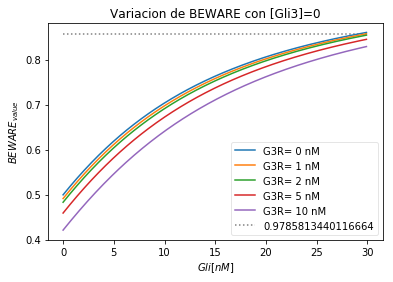
\includegraphics[width=0.8\textwidth]{variacion_new_beware}
	\centering
	\caption{Variación del nuevo operador BEWARE }
	\label{vari_beware}
\end{figure}

\begin{figure}[h]
	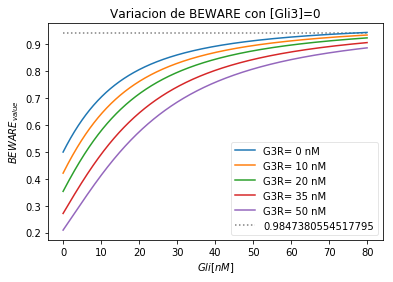
\includegraphics[width=0.8\textwidth]{variacion_new_beware_2}
	\centering
	\caption{Variación del nuevo operador BEWARE en más rango}
	\label{vari_beware_2}
\end{figure}

\subsection{Evolución temporal}

\begin{figure}[h]
	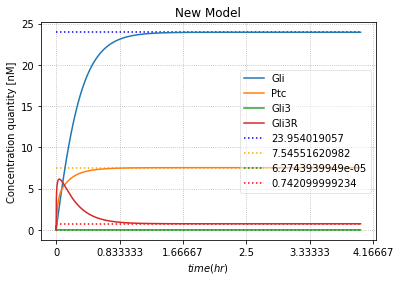
\includegraphics[width=0.8\textwidth]{new_beware_global}
	\centering
	\caption{Evolución temporal del nuevo operador BEWARE}
	\label{evolu_beware}
\end{figure}

\subsection{Análisis numérico de los estados estacionarios}


